\chapter{Physics Formalism}
\label{ch:physrev}
Talk about the development of current physics that describes nuclear and particle physics from the development of quantum physics to quantum electrodynamics and quantum chromodynamics.

\section{Nucleon Structure}
The proton and neutron are the two components that make up a group called nucleons since they are the only two particles that make up the nucleus of an atom. The both interact through all four forces ($i.e.$ strong nuclear, weak nuclear, electromagnetic, and gravitational). As mentioned in the Introduction, they are both fermions. Because they are both made up of three quarks, they are also both baryons.

The quarks that make up these nucleons (all baryons, in fact) and that are responsible for their quantum numbers are called $valence$ $quarks$. The proton is made of two $up$ valence quarks and one $down$ valence quark, denoted by $uud$. The neutron is made up of two down valence quarks and an up valence quark, or $udd$. Of course, there are also $sea$ $quarks$ made of $q\bar{q}$ pairs, where $q\bar{q}$ is any variety of quark-antiquark pair. However, the strong interaction which binds all of these quarks together acts the same no matter the quark flavor\footnote{The word \textit{flavor} is used to describe a type of quark. Remember there are 6 \textit{flavors} of quarks: up, down, top, bottom, strange, and charm.}. Therefore, the quark model does not predict any distinctions between protons and neutrons. In fact, from the view of the strong force, they are the identical particle in different states\footnote{There is a symmetry of the strong interaction in neutrons and protons called isospin (also referred to as isotopic or isobaric spin). Isospin is a dimensionless quantity that is not describe a physical "spin" of the particle. It does, however, offer a description of the two different states of nucleons. In particular, the projection of isospin along the z-axis ($I_z$ or $I_3$) provides insight into the difference between protons and neutrons, which are otherwise almost identical particles. Protons have $I_z=1/2$ and neutrons have $I_z=-1/2$.}. Yet, protons and neutrons are clearly not identical particles.

There are obvious differences between two nucleons. One important difference between nucleons is their stability when not bound to each other. The proton is a stable particle on its own, with a lifetime of more than $2.1 \times 10^{29}$ years. The neutron, however, has a lifetime of about $882$ seconds (or about 15 minutes). The proton is the only nucleon that can exist in a nucleus on its own, such as in the hydrogen atom. Yet, the obvious difference in the two nucleons is their electric charge. The charge of the proton is $+1$ in units of electron charge, while the neutron is neutral ($i.e.$ charge = 0). This charge arises from their valence quark content. The up quark has a charge equal to $q_u = +2/3$ and the down quark has a charge of $q_d = -1/3$, so for the proton with $uud$ quarks

\begin{equation}
2q_u + q_d = 2(+2/3) + (-1/3) = +1
\end{equation}
and for the neutron with $ddu$ quarks

\begin{equation}
2q_d + q_u = 2(-1/3) + (+2/3) = 0.
\end{equation}
This charge distribution of quarks is well known for both nucleons. The momentum distribution of those quarks inside the nucleon is not as well known, especially for the neutron. The same is true for the overall structure of the nucleons, again more so for the neutron.

\begin{figure}[h!]
	\centering
	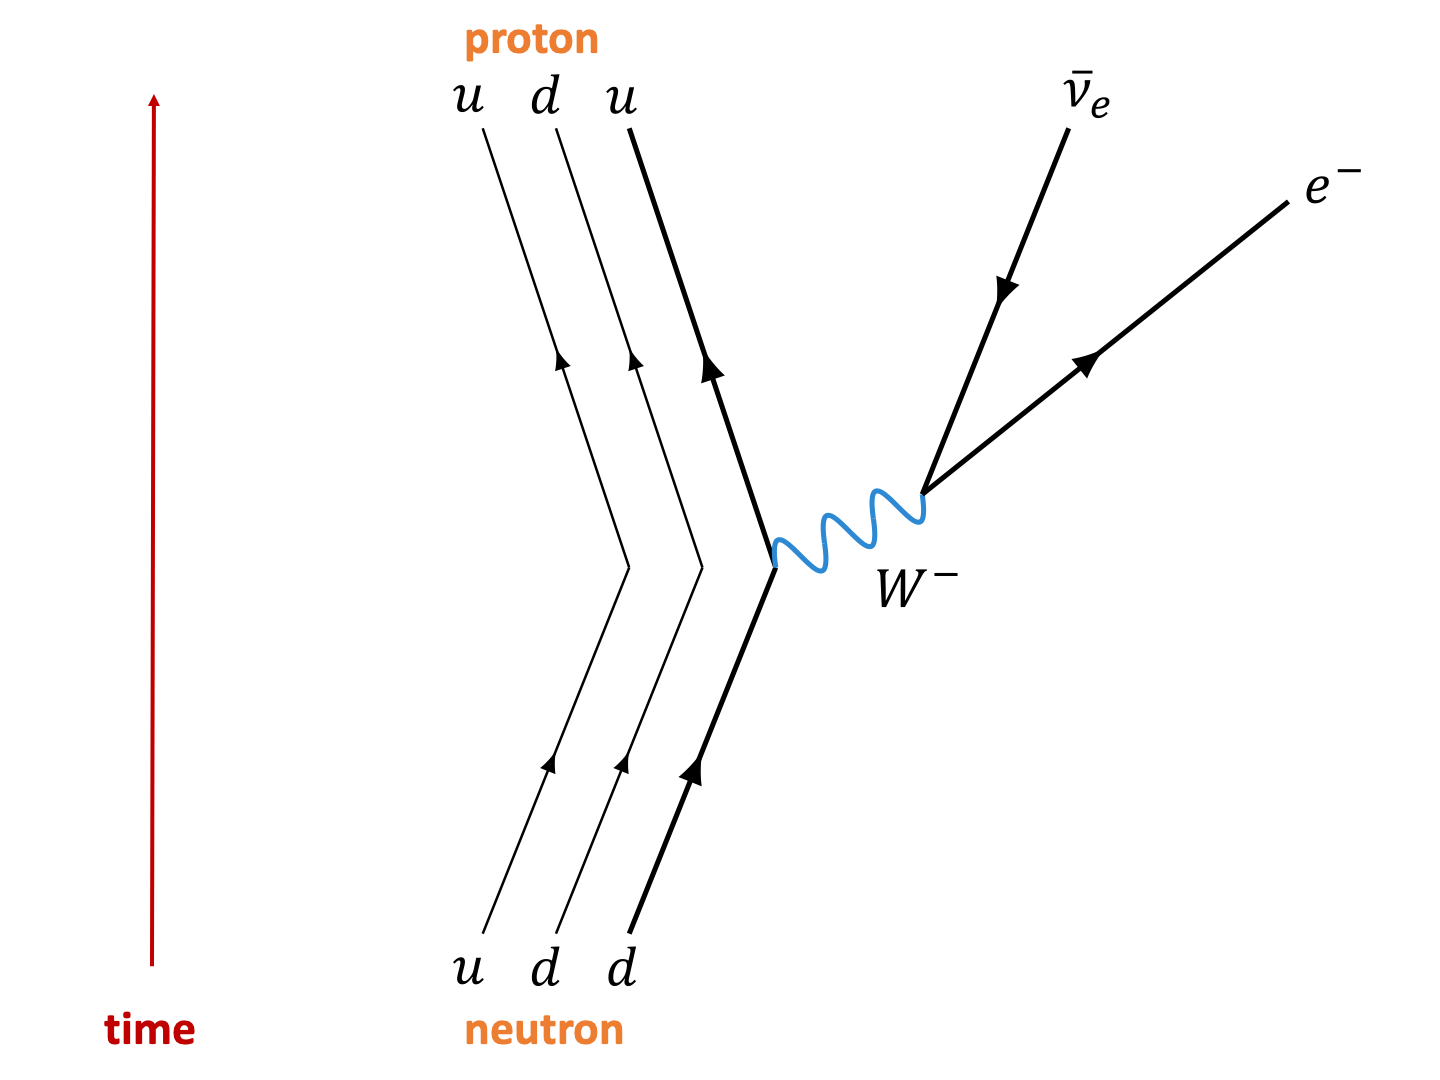
\includegraphics[width=0.6\linewidth]{figures/neutron_decay.png}
	\caption{The Feynman diagram of neutron decay.}
	\label{fig:neutron_decay}
\end{figure}

The discrepancy of knowledge between the proton and the neutron is the last major difference of the nucleons we will discuss here, because it goes directly toward the principle of the BONuS12 Experiment. We know much more about the structure of the proton and momentum distribution of the quarks inside the proton for the reason discussed in the last paragraph. That is, protons can exist outside of nuclei while neutrons soon decay via the weak interaction

\begin{equation}
n \longrightarrow p + e^{-} + \bar{\nu}_{e}
\end{equation}
seen in in Fig. \ref{fig:neutron_decay} as a Feynman diagram. Feynman diagrams were developed by physicist Richard Feynman to display particle interactions that occur in a relatively simplistic manner. Moving from the bottom to the top in the diagram of Fig. \ref{fig:neutron_decay}, we see a down quark within the neutron change states to an up quark mediated by the $W^-$ boson emitting an electron ($e^-$) and electron antineutrino ($\bar{\nu}_{e}$). This decay happens within 15 minutes of a neutron being a free particle. That decay coupled with the fact that the neutron has no electric charge makes isolating neutrons to create a target for scattering experiments extremely difficult. Yet, scattering experiments are the primary means by which physicists study the structure of particles. Therefore, studying the structure of the neutron is inherently made difficult by this lack of free neutron target.

\section{Electron-Scattering Kinematics}
To study the structure and physics of particles, nuclear and particle physicists use scattering experiments. There are two ways of creating a scattering experiment. One way is to accelerate a light particle (an electron, for example) and direct it toward a stationary target, which is the method used at Jefferson Lab in Newport News, Virginia. The other way is to accelerate two particles in opposite directions and then direct the two toward each other, which is the method used at the Large Hadron Collider (LHC) at CERN in Geneva, Switzerland. The physics or kinematics\footnote{The word kinematics refers to the mechanics of the particles without concern for the forces that caused the motion. Essentially, we are not concerned with $how$ the particles were accelerated, just that they have a particular energy at the time of collision.} of both scattering experiments is essentially the same. 

When the scattering particle and target collide, some of the momentum and energy of the scattering particle is transfered to the target particle. The way that nuclear and particle physicists express that energy and momentum is in something called its four-momentum. Classical momentum is a vector, which means it has a magnitude and direction. That direction is typically expressed in three dimensions (for the familiar Cartesian coordinate system that would be along the x, y, and z-axis). Therefore a momentum can be expressed as $\mathbf{p}$ = ($p_x$, $p_y$, $p_z$), where $\mathbf{p}$ is the momentum vector bold-faced to indicate that it is a vector. Because in particle physics, the particles travel close to the speed of light, so we have to deal with special relativity. For the purposes of this work, special relativity essentially forces us to consider not just three-dimensional space, but four dimensional space-time with different reference frames for different moving objects. This drives us to require there be a four-dimensional space-time momentum $p=(p_0,p_1,p_2,p_3)$, where $p_1=p_x$, $p_2=p_y$, and $p_3=p_z$ in Cartesian coordinates. The new term $p_0$ is equal to $E/c$, where $E$ is the energy of the particle and $c$ is the speed of light.

If we take this four-momentum
\begin{equation}
p_{\mu} = \left( \frac{E}{c}, p_x, p_y, p_z \right),
\end{equation} 
where $\mu$ is just an index indicating a particular particle and square it, we have
\begin{equation}
p^{\mu}p_{\mu} = -\frac{E^2}{c^2} + p^2_x +p^2_y + p^2_z = -\frac{E^2}{c^2} + p^2.
\end{equation}
This quantity should be invariant under a Lorentz transformation and is equal to the Lorentz scalar $-m^2c^2$, which means 
\begin{equation}
\label{eqn:4mom}
-\frac{E^2}{c^2} + p^2 = -m^2c^2.
\end{equation}
Multiplying both sides of Eq. \ref{eqn:4mom} by $-c^2$ and rearranging a little gives us
\begin{equation}
\label{eqn:e_squared}
E^2 = - p^2c^2 + m^2c^4,
\end{equation}
which if we take the square root of both sides results in
\begin{equation}
E=\sqrt{(pc)^2+(mc^2)^2}.
\end{equation}
In the rest frame of the particle ($i.e.$ the frame where the particle is considered to have no momentum, thus $p=0$), this equation reduces to something that should be familiar. That is
\begin{equation}
E=mc^2.
\end{equation}
This rough derivation provides a little insight to the power and purpose of using four-momentum. We will use this extensively throughout the rest of this work. 

The other useful notation to understand is called natural units, where $c=\hbar=1$. Under these units, Eq. \ref{eqn:e_squared} becomes
\begin{equation}
E^2 = p^2 + m^2.
\end{equation}
While this offers much in the way of simplicity when working with complex equations, the disadvantage is that we lose information regarding dimensional analysis of the equation. Nevertheless, for the most part, we will use natural units in this work.

Now, consider an electron with four-momentum $k$ scattering off of a proton with momentum $p$. The Feynman diagram for such an interaction is in Fig. \ref{fig:feyn_epscatt}, where $k'$ and $p'$ are the final momentum of the scattered electron and proton respectively. Here, $q$ is the momentum of the virtual photon\footnote{The term "virtual" here may be misleading. It does not imply that the photon does not really exist. It refers to the short-lived exchange of the electromagnetic force.} (typically denoted by $\gamma^{*}$ ) that mediates the interaction. That virtual photon momentum is defined as $q=k'-k$, which implies that it is the momentum lost by the scattered electron.

\begin{figure}[h!]
	\centering
	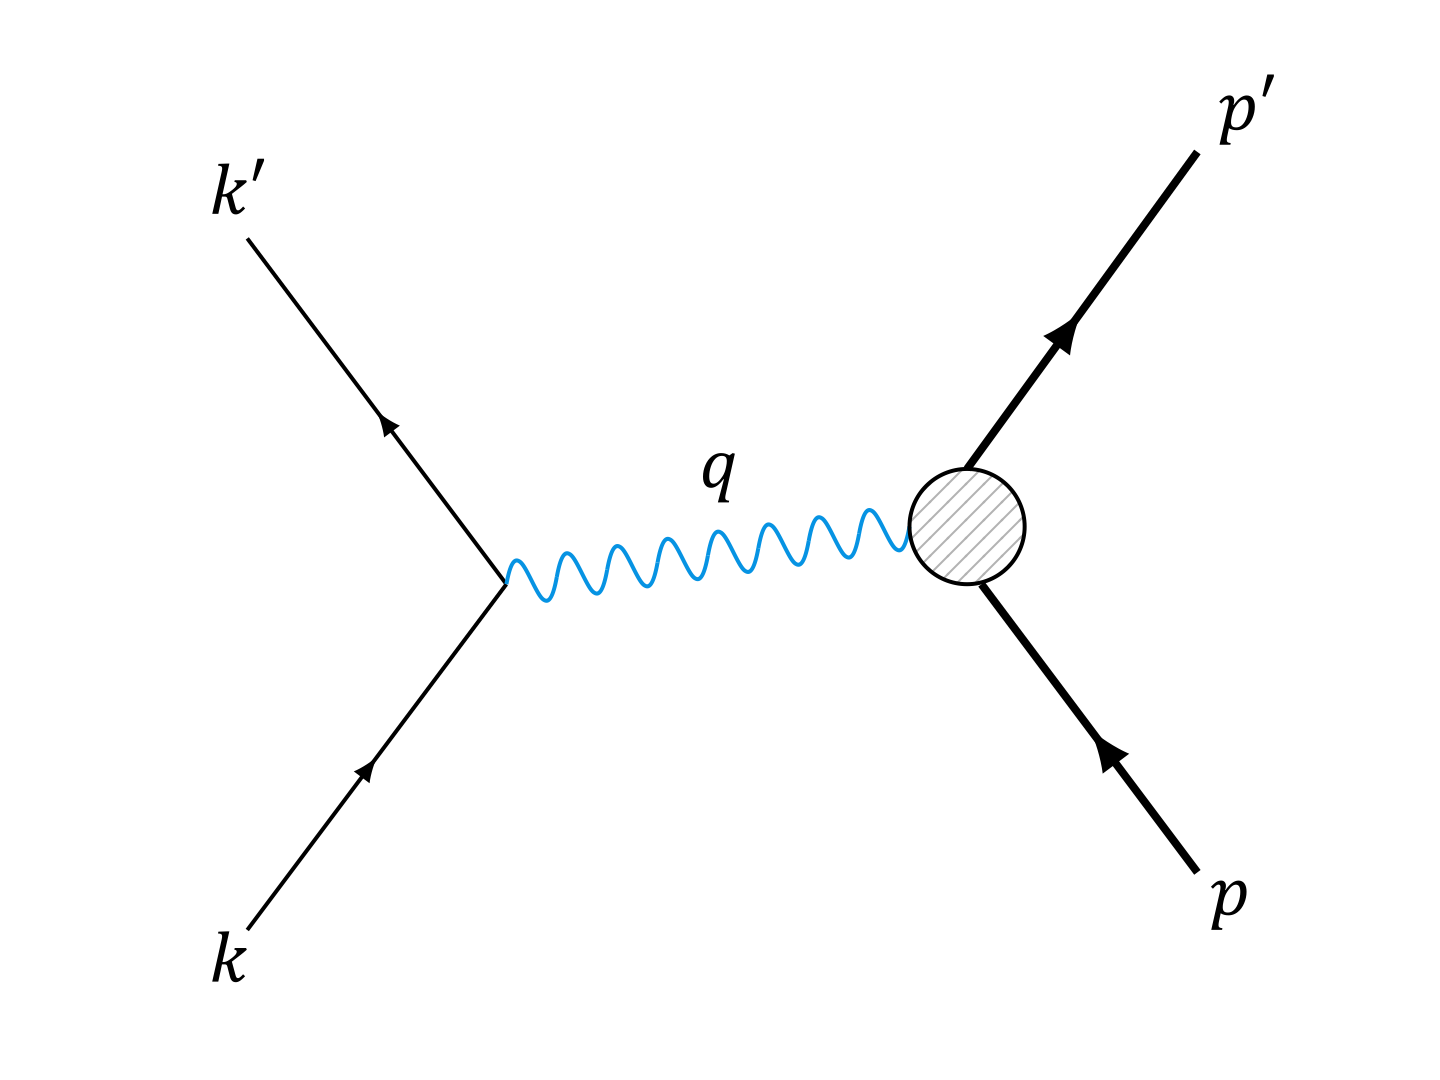
\includegraphics[width=0.6\linewidth]{figures/feyn_epscatt.png}
	\caption{Feynman diagram of an electron scattering from a proton.}
	\label{fig:feyn_epscatt}
\end{figure}

There are some other important quantities to consider for electron scattering. The first is the square of that momentum transfer
\begin{equation}
q^2 = (k' - k)^2 = 2m_e^2 - 2(EE' - |\mathbf{p}||\mathbf{p}'| \cos \theta),
\end{equation}
where $m_e$ is the mass of the electron, $E$ is the energy of the incident electron, $E'$ is the energy of the scattered electron, $|\mathbf{p}|$ is the magnitude of the three-momentum of the incident proton, $|\mathbf{p}'|$ is the magnitude of the incident proton's three-momentum, and $\theta$ is the scattering angle of the electron. When we use the trigonometric identity $1-\cos \theta = 2 \sin^2 \tfrac{\theta}{2}$ and take the electron mass to be zero, we get
\begin{equation}
q^2 \approx -4EE'\sin^2\tfrac{\theta}{2}.
\end{equation}
As a convention to make the quantity positive, we use $Q^2 = -q^2$, which will be used throughout the rest of this work. Another variable we need to analyze these electron scattering kinematics is the variable $\nu$, which is the energy transfer of the electron to the proton via $\gamma^*$ ($i.e.$ the virtual photon) and is defined by
\begin{equation}
\nu = \frac{p \cdot q}{M}.
\end{equation}
Here, $p$ is the four-momentum of the incident proton, $q$ is the four-momentum of the incident electron and $M$ is the proton mass. In the laboratory frame, the proton is at rest ($i.e.$ $p=(M,\mathbf{0})$)\footnote{Just like other three-dimensional vectors, when bolded, $\mathbf{0}$ represents (0,0,0).}, and $q=(E-E',\mathbf{q})$, so the energy transfered by the virtual photon to the proton in the laboratory frame would be
\begin{equation}
\nu  = E-E'.
\end{equation}

\begin{figure}[h!]
	\centering
	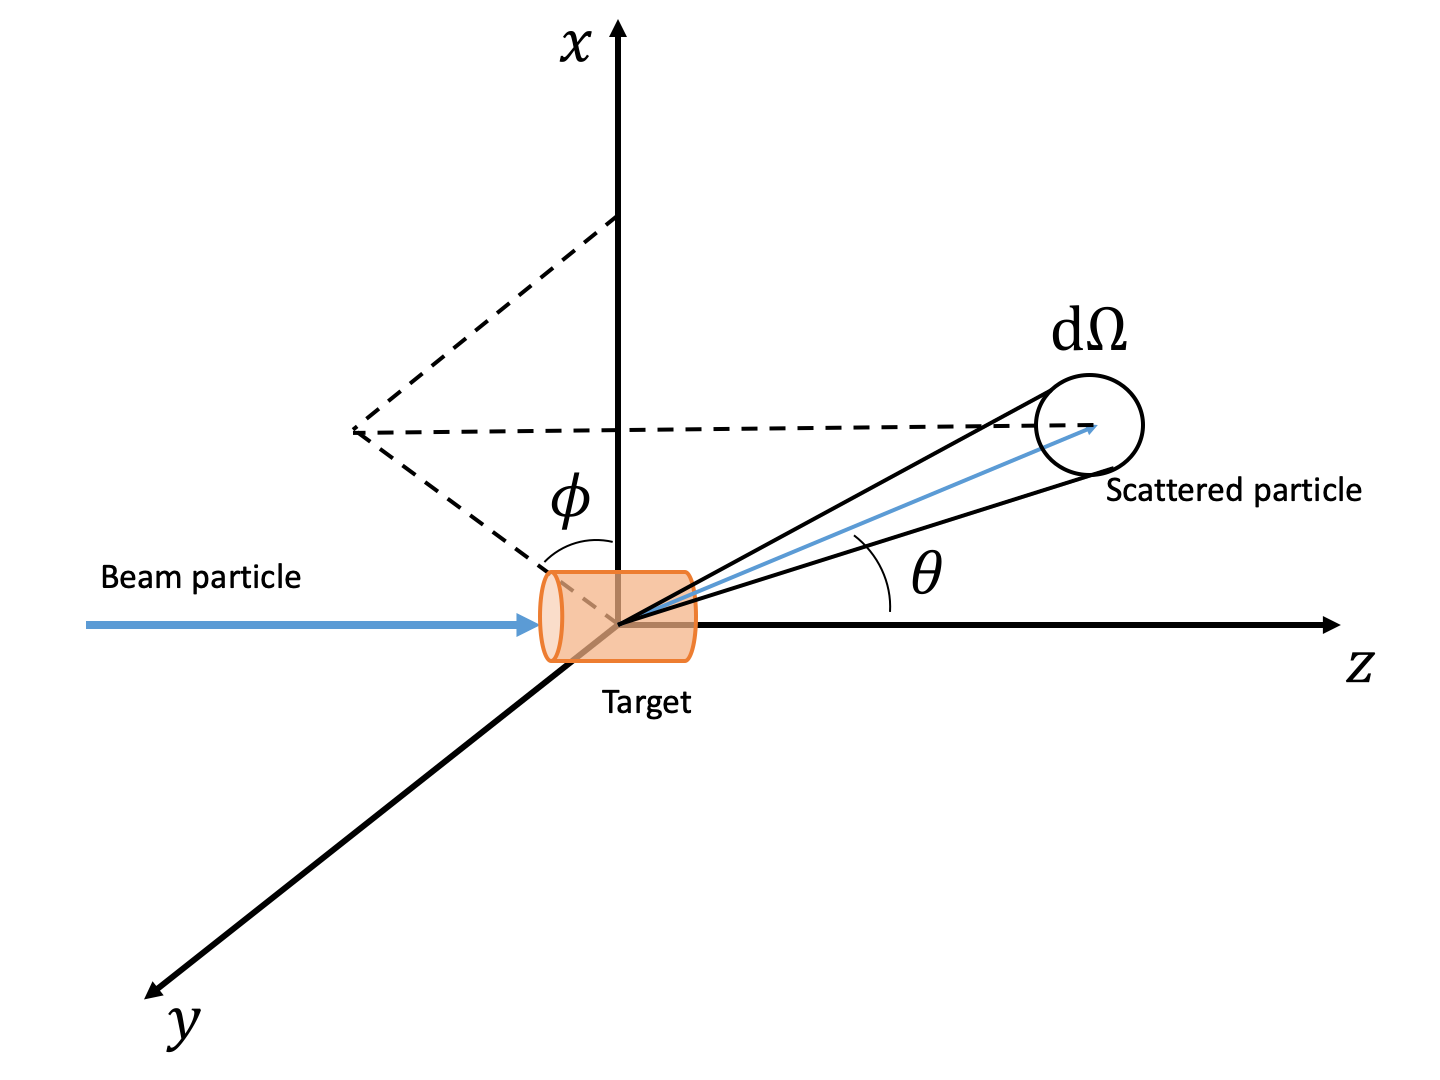
\includegraphics[width=0.6\linewidth]{figures/diff_xsec.png}
	\caption{Differential cross section.}
	\label{fig:diff_xsec}
\end{figure}

Whenever we deal with collisions of particles, there is a probability associated with the reaction between that projectile and target. That probability is called the $cross$ $section$ and with it often comes a wealth of knowledge about the dynamics of the interaction itself. In many reactions we deal with what is known as the $differential$ cross section, which offers a more realistic insight to only a fraction of reactions. 

The type of scattering depicted in Fig. \ref{fig:feyn_epscatt} is called $elastic$ $scattering$, which simply means that both particles remain intact after the collision. Like pool balls, they essentially bounce off of each other, of course through the exchange of that virtual photon. When the amount of energy transfer increases ($i.e.$ when $q$ increases), different types of scattering arise. We need to understand those types of scattering and how they arise in more depth to understand the BONuS12 Experiment.

\section{Elastic Regime}


\section{Resonance Region}
\section{Deep Inelastic Scattering}

\section{The Quark-Parton Model}
\section{Quantum Chromodynamics}
\section{Nucleon Structure-Function Ratio $F^2_n/F^2_p$}
\section{Difficulties in Extracting $F^2_n/F^2_p$ from Deuterium}
\subsection{Bound Nucleon Structure}
\subsection{Backgrounds}
\section{Barely Off-Shell Nucleon Structure}
